% TODO: figures for the following:
% - Latent dataset generation X
% - 2d aware modifications: 2d rotary embeddings and downsampling in two X
%   directions (showing failings of previous) X
% - show training procedure (original z, corruption function, unrolled
%   training). show samples at each step? or save for eval
% - show sampling procedure (random z_0, unrolled steps, show samples, binary X
%   mask) X
% - show some nice samples! X

% TODO: could use some high level diagram of the method at the start of the
% section (acting as a bit of a map)?
% TODO: also some more figures and equations to break up the walls of text.
% TODO: in general, more assertive language would be good. 

% TODO: kinda want to improve the sampling figure

\subsection{Latent Dataset Generation}
We use the standard two-stage scheme for vector-quantized image
modelling~\cite{oord2018neural,razavi2019generating,esser2021taming,bondtaylor2021unleashing}
using VQ-GAN~\cite{esser2021taming} as our feature extractor. Where such models
are available, we use pretrained \glspl{vqgan} for our experiments. For higher
resolution experiments (for example, FFHQ1024~\cite{karras2019stylebased}),
pretrained models are not available and so training our own VQ-GAN was necessary
(see \S\ref{sec:megagan}).

The second stage is to learn a discrete prior model over these latent variables.
To enable this, we first build a latent dataset using our trained \gls{vqgan}.
This allows for faster training of our second-stage model as the discrete latent
representations have been precomputed. A downside of this approach is that it
limits the amount of data augmentation that can be applied to the dataset. We
apply a simple horizontal flip to all images, effectively doubling the dataset
size. Formally, given a dataset of images
$\imageDataset$, a VQ-GAN encoder $\vqganEncoder$ with downsample factor
$\vqganDownsample$, and vector-quantization codebook $\vqganCodebook$ with
number of codewords $\vqganNbLatents$, trained on $\imageDataset$, we define our
latent dataset $\latentDataset$ as:
\begin{equation}
    \latentDataset = \{\vqganCodebook(\vqganEncoder(\image)) \mid \image \in \imageDataset \}
\end{equation}
where $\image \in \real{3 \times H \times W}$ is a single element of the
augmented image
dataset and $\latent = \vqganCodebook(\vqganEncoder(\image)) \in \{1, \dots,
\vqganNbLatents\}^{h \times w}$ is the corresponding discrete latent
representation. In other words, each $\vqganDownsample \times \vqganDownsample$
pixels in $\image$ is mapped to a single discrete value from $1$ to
$\vqganNbLatents$ (which in turn, corresponds to a vector $\codebookVector \in
\vqganCodebook$),
resulting in a latent representation of shape $\frac{H}{f} \times \frac{W}{f} =
h \times w$.

We then use $\latentDataset$ to train a discrete prior over the latents. Coupled
with the VQ-GAN decoder $\vqganDecoder$, we obtain a powerful generative model
by first sampling from a discrete uniform prior distribution, denoising using
\gls{sundae}, and then decoding the final latents using the \gls{vqgan} decoder.
Training this discrete prior model, forms the bulk of our work in this paper.

\subsection{2D-Aware Hourglass Transformer}
Inspired by successes in hierarchical transformers for generative language
modelling~\cite{nawrot2021hierarchical}, we modify their architecture for use
with discrete latent representations of image data. We will later use this
architecture to implement a discrete prior over the \gls{vqgan} latents. 

Hourglass transformers have been shown to efficiently handle long-sequences,
outperform existing models using the same computational budget, and meet the
same performance as existing models more efficiently by using an explicit
hierarchical structure~\cite{nawrot2021hierarchical}. The same benefits should
also apply to vector-quantized image modelling. 

However, the design and parameters chosen by the original authors were tailored
for language modelling. They also experimented with pixel-wise image
generation, though we believe that we can improve upon their architectural
choices for the task of discrete latent modelling. Some changes may also be
applicable to direct image modelling. We outline modifications to the
architecture in this subsection.

% TODO: add a figure demonstrating this
\textbf{2D-Aware Downsampling} -- The original formulation of hourglass
transformers~\cite{nawrot2021hierarchical} introduced both upsampling and
downsampling layers, allowing the use of hierarchical transformers in tasks that
have output sequence lengths equal to the input sequence lengths. However,
applying their proposed resampling strategies directly on the vector-quantized
image may not be the best strategy. 

In their work, resampling is applied to the flattened embedding sequences,
meaning that the corresponding two-dimensional vector-quantized image is
actually resampled more in one axis compared to the other. In their work they
did not address this, except for experiments on
ImageNet32~\cite{russakovsky2015imagenet} where they resampled with a rate of
$\hourglassRate=3$, corresponding to three colour channels. However, if they
were to nest the hourglass transformers further, they would encounter this issue
of one spatial dimension being downsampled more than others.

\begin{figure}[ht!]
    \label{fig:resample}
    \centering
    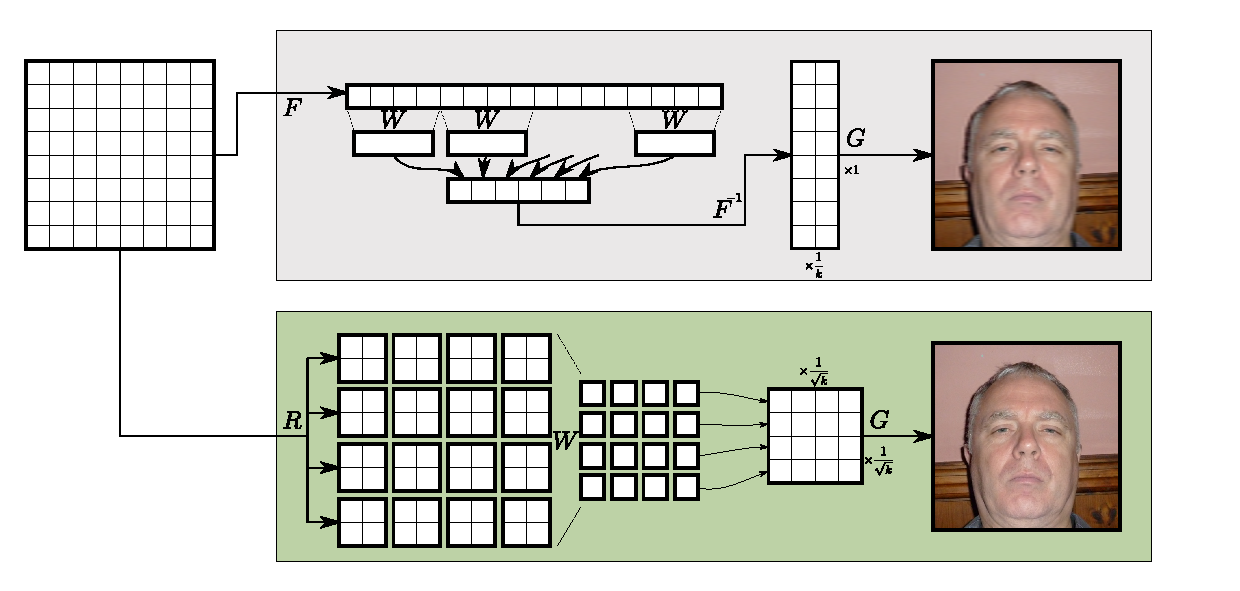
\includegraphics[width=\textwidth]{figures/resample.pdf}
    \caption{
        \textbf{Top:} Showing effect of resampling sequence embeddings using
        original formulation. Resampling rate will be applied to only one axis,
        resulting in resampling more in only one axis of the decoded image.
        \textbf{Bottom:} Our corrected method of resampling, extracting first
        two-dimensional patches of size $\sqrt{\hourglassRate}$, then applying
        resampling. The sequence can then again be flattened and passed to
        subsequent transformer layers.
    }
\end{figure}

In our formulation, we instead reshape the flattened sequence back into a
two-dimensional form and then apply resampling equally in the last two axes.
With a resampling rate of $\hourglassRate$ we apply $\sqrt{\hourglassRate}$ in
each axis -- evenly distributing the resampling among the axes. In our
preliminary experiments, we found this to significantly improve the performance
of the discrete prior model, and suspect a similar approach could improve
performance if applied to pixels directly, which we leave for future work to
confirm.

For all experiments we use the linear resampling method proposed
in~\cite{nawrot2021hierarchical} as this was the recommended option for image
data. In addition, attention layers are applied directly after resampling as
this led to best results on both image and text datasets in the original
work~\cite{nawrot2021hierarchical}. This means our adjusted resampling method is
as follows:
\begin{equation}
    h' = A(\hourglassResample^{(\intercal)} \cdot R(\vh) + \vr), \;\; \hourglassResample \in
    \mathbb{R}^{\frac{(d \cdot h \cdot w)}{\hourglassRate} \times (d \cdot h \cdot w)}
\end{equation}
where $A$ is the post-resampling attention layer, $\vh$ is the current hidden
state, $\vr$ is the residual (with $\vr = \bm{0}$ when downsampling), $R$ is the
modified reshape operation, $d$ is the hidden layer dimension, and $W$ is a
learned projection matrix. The reshape operation $R$ can be implemented as a
space-to-depth operation followed by combining the feature and depth dimensions.

\textbf{Rotary Positional Embeddings}~\cite{su2021roformer} are a good default
choice for injecting positional information into transformer models, requiring
no additional parameters. Additionally, they can be easily extended to the
multi-dimensional case~\cite{rope-eleutherai} which we do here. Though
transformers are clearly capable of learning that elements far apart in a
flattened sequence may be close in a multi-dimensional final output, we found
that explicitly extending positional embeddings to the multi-dimensional case to
provide a modest boost in performance. The original hourglass transformer on
pixel-wise generation also opted to use rotary
embeddings~\cite{nawrot2021hierarchical}. They note also that rotary embeddings
have the advantage of being compatible with any self-attention mechanism.

\textbf{Removal of Causal Constraints} -- In the original autoregressive
formulation of hourglass transformers, great care was taken to avoid information
leaking during resampling, and hence making the model
non-causal~\cite{nawrot2021hierarchical}. We use a non-autoregressive method
which is therefore not causal. Hence, in our approach we do not make any special
considerations to avoid information leaking into the future. This simplifies the
model by avoiding the ``shifting'' operation required in the original work.

\subsection{Training a megapixel VQ-GAN}
\label{sec:megagan}
% TODO: details about FFHQ1024 VQGAN.
% this kind of stuff might be better in "evaluation" though

\begin{figure}[ht]
    \centering
    \includegraphics[width=\textwidth]{figures/recon.pdf}
    \caption{
        \gls{vqgan} does not produce entirely faithful reconstructions due to
        being optimised for perceptual quality rather than a direct error between
        the reconstructions and inputs. The top row shows example inputs, middle row
        shows resulting reconstructions, and the final row shows points of interest that
        have been modified -- some perceptually valid and others clear
        artifacts. 
        \textbf{Left}: The eye colour has been brightened, and hair
        shifted to conceal a piercing, rather than reconstruct it.
        \textbf{Middle}: The most common reconstruction artifact occurs with
        certain types of hair, where a repeating and unrealistic pattern occurs. The
        pose of the lip is also altered. 
        \textbf{Right}: Another common artifact where text in images is
        corrupted. This is common across many generative models. Additionally,
        the model removes nose and lip piercings, in addition to altering eye
        makeup. This is again a valid image, but does not faithfully reconstruct
        the input.}
\end{figure}

Training at higher resolutions usually means greater computational requirements
and sampling speeds. With an autoregressive model, the sampling speed can be
especially immense, even with an auxiliary vector-quantized image
model~\cite{esser2021taming}. With a non-autoregressive model however, one
question to explore is whether sampling at very high resolutions becomes
feasible.

To answer this question, we train a larger variant of VQGAN with
$\vqganNbLatents = 8192$ operating on $1024 \times 1024$ RGB images. To our
knowledge, this is the highest resolution VQGAN has been applied
to~\cite{esser2021taming}. Once trained, can generate a latent datasets as
before, the only difference being an increased sequence length -- greater than
was ever tested in the original work~\cite{savinov2022stepunrolled}.
Specifically, we obtain a downsampling rate of $\vqganDownsample=32$, resulting
in discrete latent size of $32 \times 32 = 1024$.

% TODO: add figure showing some artifacts in reconstructions
The resulting reconstructions are overall of good quality given the relatively
extreme compression ratio we are using. However, certain artifacts in the
reconstructions still remain, particularly with certain hair types, facial
features, and uncommon accessories. Examples of such artifacts are shown in
Figure~$i$.

% TODO: add gpu specification
Using vector quantized image modelling to compress images further whilst
retaining high quality and faithful reconstructions remains an open and
challenging area of research. In our case at very high resolutions, this is
especially true. In our preliminary experiments, we found a higher
$\vqganDownsample$ led to the average reconstruction being of very poor quality.
Conversely, decreasing $\vqganDownsample$ led to latent representations of sizes
that led to large memory requirements in the downstream \gls{sundae} prior.
Furthermore, training \gls{vqgan} at this resolution is extremely
computationally expensive -- in our configuration being limited to a total batch
size of 4 across four GPUs. This made a full hyperparameter sweep of the other
parameters of the model not possible. Therefore, we decided to compromise with
good reconstructions on average, and accept occasional artifacts which could 
potentially manifest in the final samples.

\subsection{Non-Autoregressive Generator Training}

% TODO: more details on generator training

We train a SUNDAE model on the flattened extracted \gls{vq} latents $\latent =
\{\latent^{(0)}, \dots, \latent^{(N)}\}$ where $N = \latentHeight \cdot \latentWidth$.
The function $\sundae(\cdot)$ is implemented using our proposed 2D-aware
hourglass transformer. The \gls{vq} are flattened in a raster-scan format and
did not experiment with other flattening techniques.

Given a latent $\latent$, we first apply our corruption distribution. This is
done by first sampling a corruption threshold vector $\corruptionThreshold$ with
$\corruptionThreshold_i \sim U[0, 1]$ and a random matrix $\mathbf{R}$ of the
same shape as $\latent$ where $R_{i,j} \sim U[0,1]$. Using this, we construct a
mask matrix $\mathbf{M}$ with $M_{i,j} = 1$ when $R_{i,j} < t_i$ and $0$
otherwise. This results in $\mathbf{M}_i$ having approximately
$\corruptionThreshold_i$ of its entries be $1$.

Then, given $\latent_0 \sim p_0$, we compute a new $\latent_0$ to start unrolled
denoising from:
\begin{equation}
    \latent_0 \leftarrow \mathbf{M} \cdot \latent_0 + (\mathbf{1} - \mathbf{M})
    \cdot \latent \text{.}
\end{equation}

We then iteratively unroll the current sample $\latent_{t-1}$ to obtain
$\latent_t$ for steps $t\in \{1, \dots, \markovSteps\}$. To perform one unroll
step, simply compute logits $\sundae(\latent_t \vert \latent_{t-1})$ and then
sample from the resulting distribution to obtain $\latent_t$, storing the logits
at each step. Then, compute the cross entropy loss between all logits at each
$t$ and the target $\latent$. This differs from some other \gls{nar} solutions
which predict the corruption noise $\epsilon$~\cite{ho2020ddpm} rather than the
target itself. The mean of the cross entropy losses is then to produce the final
loss as shown in \S\ref{subsec:sundae}, which then allows for backpropagation
of gradients.

Though the default $\markovSteps = 2$ performed well, we found $\markovSteps =
3$ to result in more diverse samples in certain experiments.

\begin{table}
    \centering
    \begin{tabular}{|c||c c||c||c c||c||}
    \hline
    \textbf{Dataset} & \textbf{FFHQ-256} & \textbf{FFHQ-1024} & \textbf{CelebA}
                     & \textbf{MNIST} & \textbf{FashionMNIST} &
                     \textbf{ImageNet} \\
    \hline
    Dataset Size & $60,000$ & $60,000$ & $190,000$ & $60,000$ & $60,000$ & $1.28$M \\
    Codebook Size & $1024$ & $8192$ & $1024$ & $256$ & $256$ & $1024$ \\
    Latent Shape & $16 \times 16$ & $32 \times 32$ & $16 \times 16$ & $28 \times
                 28$ & $28 \times 28$ & $16 \times 16$ \\
    Unroll Steps & 3 & 3 & 3 & 2 & 2 & 3 \\
    \hline
    Depth & $3-10-3$ & $2-12-2$ & $2-12-2$ & $2-8-2$ & $2-8-2$ & $3-14-3$\\
    Dimension & 1024 & 1024 & 1024 & 1024 & 1024 & 1024 \\
    Shorten Factor & 4 & 4 & 4 & 4 & 4 & 4 \\
    Attention Heads & 8 & 8 & 8 & 8 & 8 & 12 \\
    Resample Type & Linear & Linear & Linear & Linear & Linear & Linear \\
    \hline
    Classes & -- & -- & -- & 10 & 10 & 1000 \\
    Class Dimension & -- & -- & -- & 1024 & 1024 & 1024 \\
    \hline
    \end{tabular}
    \caption{
        Table of parameters for all training experiments. Depth is
        represented as three numbers corresponding to number of layers before
        downsampling, number of downsampled layers, and number of layers after
        upsampling. The dataset size is the size of the training split of the
        dataset. The latent shape of MNIST experiments is exactly equal to the
        shape of $\image$, as for these experiments we operate directly on a
        (discretized) pixel-level.
    }
\end{table}
An alternative corruption distribution would be to instead use a deterministic
method $\latent_0^{(i)}=\texttt{[MASK]}$, essentially replacing all tokens with
$M_{i,j} = 1$ with a special masking token. This bears some similarity to
``progressive unmasking'' of latents as shown in prior
work~\cite{bondtaylor2021unleashing,austin2021structured}. This strategy was not
considered due to the use of a masking token places an upper bound on the number of
inference time sampling steps (updating at most one token per step) as well as
not allowing for self-correction, as once a token is unmasked it is now
fixed~\cite{bondtaylor2021unleashing,austin2021structured}. 

% TODO: a figure could be really nice too.

\subsection{Generating High-Resolution Images}
% TODO: discuss our various sampling strategies and any additional findings over
% original SUNDAE

% TODO: we found the best sampling parameters to be a little different to their
% one.
% TODO: also discuss annealing temperature, low temperature but fast, high
% temperature but slower, etc.
% in general, the sampling process for SUNDAE is highly tuneable, and probably
% dataset dependent..
% we also stop early if nothing has changed.

\begin{figure}[ht]
    \label{fig:sampling}
    \centering
    %\includegraphics[width=0.9\linewidth]{figures/sampling/sampling.pdf}
    \begin{overpic}[percent,grid=false,tics=2,width=0.9\linewidth]{figures/sampling/sampling.pdf}
        \put(6, 3){\tiny$\latent_0 \sim U(1, v)$}
        \put(31, 3){\tiny$\latent_1$}
        \put(66, 3){\tiny$\latent_{T-1}$}
        \put(88, 3){\tiny$\latent_T$}
        \put(10, 31){$\vqganDecoder$}
        \put(31, 31){$\vqganDecoder$}
        \put(67, 31){$\vqganDecoder$}
        \put(88, 31){$\vqganDecoder$}
        \put(48, 16){$\dots$}
        \put(9, 60){\tiny$\sample_0$}
        \put(31, 60){\tiny$\sample_1$}
        \put(67, 60){\tiny$\sample_{\markovSteps - 1}$}
        \put(88, 60){\tiny$\sample_\markovSteps$}
    \end{overpic}

    \caption{The sampling process. SUNDAE gradually denoises from $\latent_0$ to
    the final sample $\latent_\markovSteps$. At each step, it is possible to
    decode with $\vqganDecoder$ to produce a final image.}
\end{figure}

During sampling, we simply sample sequentially $\latent_t \sim \sundae(\latent_t
\vert \latent_{t-1})$ for a constant number of steps $\markovSteps$, beginning
randomly from $\latent_0$~\cite{savinov2022stepunrolled}. The original work
proposed a number of improved strategies for sampling in smaller number of
steps, including low-temperature sampling and updating a random subset of
tokens~\cite{savinov2022stepunrolled}, rather than all simultaneously.

Sampling, however, with a lower temperature can reduce the diversity of the
resulting samples. To alleviate this, we instead anneal the temperature down
from a high value ($\approx 1.0$) down to a lower value towards the end of the
sampling process. We found this retained the fast sampling speed whilst also
improving diversity.

In certain latent sampling configurations, updating only a random subset of
tokens does improve performance. However, we found that for low step scenarios
($\markovSteps<20$) that all tokens must be able to be updated in order to
produce meaningful samples before the maximum number of steps is reached. Hence
in these cases, we do not follow this strategy.

Additionally, if a individual sample does not change between step $t-1$ and $t$,
we freeze it, preventing any further change. If all samples are frozen, sampling
may terminate early, further improving sampling speed with little cost to
sample quality. This is significant when performing large-batch sampling.

Once sampling has terminated, the sampled latent code $\latent_T$ can be given
to the VQGAN decoder $\vqganDecoder$ to produce a final sample $\sample$.

\subsection{Arbitrary Pattern Inpainting}
% TODO: discuss how to inpaint with a trained model
% TODO: add more citations in general for other NAR
% TODO: clear advantage of NAR models against AR, as we are not limited to
% causal inpainting
% TODO: initial description may be more suited for prior work.

As noted in the original work~\cite{savinov2022stepunrolled} and other
non-autoregressive solutions~\cite{bondtaylor2021unleashing} one clear advantage
of non-autoregressive models is that they are not limited to causal inpainting.
In general, they support arbitrary inpainting masks and can draw on context in
both the past and the future, enabling them to perform inpainting tasks not
possible with autoregressive sampling.

Given a sampled image $\sample \in \real{H \times W \times 3}$ we can mask a
proportion of it using a pixel-level binary mask $\pixelMask \in \{0, 1\}^{H
\times W}$. By taking $\vqganDownsample \times \vqganDownsample$ regions of
$\pixelMask$ and applying a logical and in them, we can obtain a latent level
mask $\vqMask \in \{0,1\}^{h \times w}$. We then sample as normal from the
latents, allowing the model full context, but only update regions that were
masked according to $\vqMask$. Like with sampling, we then use $\vqganDecoder$
to decode the sampled latent code, producing the output $\sample$.
